\documentclass[aguposter,landscape]{baposter}

%\usepackage{mathpazo} % math & rm
%\linespread{1.0}        % Palatino needs more leading (space between lines)
%\usepackage[scaled]{helvet} % ss
%\usepackage{courier} % tt
%\usepackage{bookman}
\usepackage{times}
%\normalfont
%\usepackage{ae}

\usepackage[vlined]{algorithm2e}
\usepackage{url}
\usepackage{graphicx}
\usepackage{amsmath}
\usepackage{amssymb}
\usepackage{relsize}
\usepackage{multirow}
\usepackage{booktabs}

\usepackage{multicol}
\usepackage{enumitem}

\usepackage{natbib}
\usepackage{wrapfig}

\graphicspath{{Figures/}}

 %%%%%%%%%%%%%%%%%%%%%%%%%%%%%%%%%%%%%%%%%%%%%%%%%%%%%%%%%%%%%%%%%%%%%%%%%%%%%%%%
 % Multicol Settings
 %%%%%%%%%%%%%%%%%%%%%%%%%%%%%%%%%%%%%%%%%%%%%%%%%%%%%%%%%%%%%%%%%%%%%%%%%%%%%%%%
 \setlength{\columnsep}{0.75em}
 \setlength{\columnseprule}{0mm}

 %%%%%%%%%%%%%%%%%%%%%%%%%%%%%%%%%%%%%%%%%%%%%%%%%%%%%%%%%%%%%%%%%%%%%%%%%%%%%%%%
 % Save space in lists. Use this after the opening of the list
 %%%%%%%%%%%%%%%%%%%%%%%%%%%%%%%%%%%%%%%%%%%%%%%%%%%%%%%%%%%%%%%%%%%%%%%%%%%%%%%%
 \newcommand{\compresslist}{%
 \setlength{\itemsep}{1pt}%
 \setlength{\parskip}{0pt}%
 \setlength{\parsep}{0pt}%
 }

%%%%%%%%%%%%%%%%%%%%%%%%%%%%%%%%%%%%%%%%%%%%%%%%%%%%%%%%%%%%%%%%%%%%%%%%%%%%%
%% Begin of Document
%%%%%%%%%%%%%%%%%%%%%%%%%%%%%%%%%%%%%%%%%%%%%%%%%%%%%%%%%%%%%%%%%%%%%%%%%%%%%
\begin{document}
%%%%%%%%%%%%%%%%%%%%%%%%%%%%%%%%%%%%%%%%%%%%%%%%%%%%%%%%%%%%%%%%%%%%%%%%%%%%%
%% Here starts the poster
%%---------------------------------------------------------------------------
%% Format it to your taste with the options
%%%%%%%%%%%%%%%%%%%%%%%%%%%%%%%%%%%%%%%%%%%%%%%%%%%%%%%%%%%%%%%%%%%%%%%%%%%%%
\begin{poster}{
 % Show grid to help with alignment
 grid=no,
 % Column spacing
 colspacing=1.5em,
 % Color style
 headerColorOne=cyan!05!white!95!black, %white, %cyan!20!white!90!black,
 borderColor=cyan!30!white!90!black,
 % Format of textbox
 textborder=faded,
 % Format of text header
 headerborder=open,
 headershape=roundedright,
 headerfont=\Large\sf\textbf,
 background=none,
 bgColorOne=cyan!10!white,
 headerheight=0.12\textheight,
 eyecatcher=yes
}
 % Eye Catcher
{
%       \includegraphics[width=0.08\linewidth]{track_frame_00010_06}
%       \includegraphics[width=0.08\linewidth]{track_frame_00450_06}
%       \includegraphics[width=0.08\linewidth]{track_frame_04999_06}
}
% Title
{\sf \Large%Sans Serif
  \textbf{
    \textcolor{gray}{V51D-2704 }\hspace{3em}
%    {Bounds on fault strength based on simulation of rider block structures\\ emerging from brittle lithosphere extension}\hspace{2em}
     {\LARGE Numerical investigation of the morphological transition of submarine lava flow due to slope change}
     \hspace{3em}\textcolor{gray}{V51D-2704 }
  }
}
% Authors
{\sf %Sans Serif
  % Serif
  \vspace{0.5em} Eunseo Choi$^{1*}$, Masako Tominaga$^{2}$, Michael Grant Baker$^{2}$, Dave May$^{3}$, Eisuke Fujita$^{4}$ and Tomofumi Kozono$^{4}$ \\\vspace{0.5em}
  { \normalsize \hspace{0em} $^{*}$Email: \texttt{echoi2@memphis.edu} \quad $^{1}$Center for Earthquake Research and Information, University of Memphis, Memphis, TN 38152, United States. \\ \hspace{0em}
   $^{2}$Dept. of Geological Sciences, Michigan State University, East Lansing, MI, United States. \quad
   $^{3}$Institute of Geophysics, ETH Zurich, 8092, Zurich, Switzerland. \quad
   $^{4}$NIED, Tsukuba, Japan.
  }
}

%% University logo
% {
%   \begin{tabular}{r}
%     \includegraphics[height=0.12\textheight]{GFDLogohres.pdf}
%%     \raisebox{0em}[0em][0em]{\includegraphics[height=0.03\textheight]{GFD\_Logo\_hres.pdf}}
%   \end{tabular}
% }

%%%%%%%%%%%%%%%%%%%%%%%%%%%%%%%%%%%%%%%%%%%%%%%%%%%%%%%%%%%%%%%%%%%%%%%%%%%%%%
%%% Now define the boxes that make up the poster
%%%---------------------------------------------------------------------------
%%% Each box has a name and can be placed absolutely or relatively.
%%% The only inconvenience is that you can only specify a relative position 
%%% towards an already declared box. So if you have a box attached to the 
%%% bottom, one to the top and a third one which should be inbetween, you 
%%% have to specify the top and bottom boxes before you specify the middle 
%%% box.
%%%%%%%%%%%%%%%%%%%%%%%%%%%%%%%%%%%%%%%%%%%%%%%%%%%%%%%%%%%%%%%%%%%%%%%%%%%%%%

%%%%%%%%%%%%%%%%%%%%%%%%%%%%%%%%%%%%%%%%%%%%%%%%%%%%%%%%%%%%%%%%%%%%%%%%%%%%%%
  \headerbox{Abstract}{name=abstract,column=0,row=0,span=1}{
%%%%%%%%%%%%%%%%%%%%%%%%%%%%%%%%%%%%%%%%%%%%%%%%%%%%%%%%%%%%%%%%%%%%%%%%%%%%%%
\begin{center}

\begin{minipage}[t]{0.95\linewidth}
\begin{multicols}{2}
We numerically investigate the effects of variations in slope angle on the morphological transition of submarine lava flow. GALE, an open-source code for long-term geodynamic modeling, has been adapted to submarine lava flow simulations. Using the adapted GALE, we first numerically reproduce pillow lavas as accumulated tubular flows, the dominant formation process observed in nature. We then test whether an increase in slope angle causes the sheet-to-pillow transition. This specific morphological transition has been observed while the existing theory and analogue models for lava flow morphology predict the opposite. The combined effects of a slope angle change and other lava source parameters (e.g., effusion rate) on lava morphology are also modeled. Finally, the model results and performance of the adapted GALE are benchmarked against pTatin3d, a finite element marker-and-cell based library developed for studying large deformation processes of very viscous fluids.
\end{multicols}
\end{minipage}

\end{center}

}

%%%%%%%%%%%%%%%%%%%%%%%%%%%%%%%%%%%%%%%%%%%%%%%%%%%%%%%%%%%%%%%%%%%%%%%%%%%%%%
  \headerbox{Submarine Lava Flow Morphology}{name=morphology,column=0,below=abstract,span=1}{
%%%%%%%%%%%%%%%%%%%%%%%%%%%%%%%%%%%%%%%%%%%%%%%%%%%%%%%%%%%%%%%%%%%%%%%%%%%%%%
     \begin{minipage}[t]{0.49\linewidth}
      $\diamond$ Dimensional analysis of solidifying flows with constant effusion rate gives two independent dimensionless parameters \citep{Fink1990}:
      \begin{itemize}
        \item Normalized temperature: $\Theta_{s}=(T_{s}-T_{a})/(T_{l}-T_{a})$ where $T_{l}$ is the temperature of lava, $T_{s}$ is the solidification temperature and $T_{a}$ is the ambient temperature.
        \item Modified P\'{e}clet number: $Pe=UH/\kappa$, where $U$ is the lateral velocity scale, $H$ is the depth scale and $\kappa$ is the heat diffusivity.
      \end{itemize}
      $\diamond$ More importantly, these two parameters can be combined into one, $\Psi$:
      %\vspace{-1em}
      \setlength{\abovedisplayskip}{0em}
      \setlength{\belowdisplayskip}{0em}
      \[ \Psi = t_{s}/t_{a},\]
      where $t_{s}$ is time for the onset of solidification of an element of lava after brought into contact with the environment and $t_{a}$ is timescale for lateral advection of viscous fluid in the absence of cooling.
    \end{minipage}
    \begin{minipage}[t]{0.49\linewidth}
      \begin{center}
        \vspace{-0.5em}
        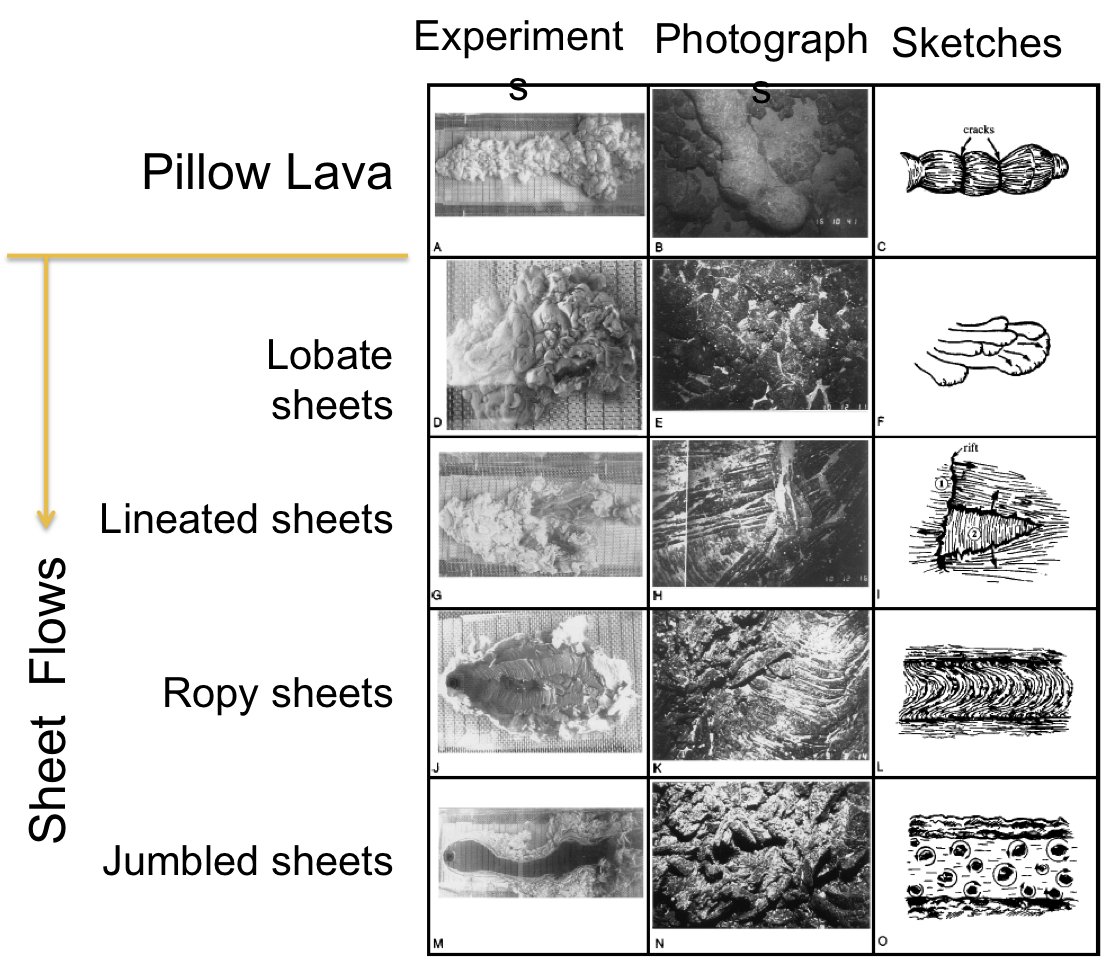
\includegraphics[width=0.9\textwidth]{lavamorphology02_GreggFink_Geology_1995.png}
      \end{center}
      \vspace{0.5em}
      \begin{center}
        \vspace{0.5em}
        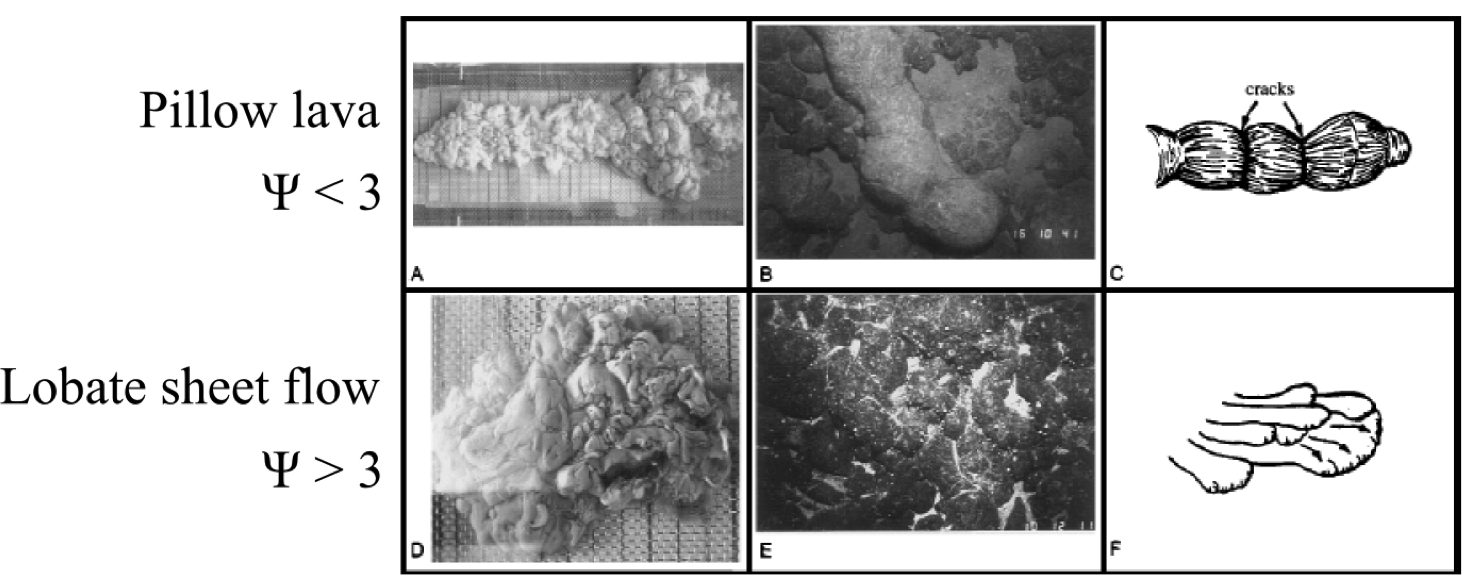
\includegraphics[width=0.9\textwidth]{lavamorphology03_GreggFink_Geology_1995.png}
        \citep{Gregg1995}
      \end{center}
      
      \vspace{0.5em}
    \end{minipage}
}

%%%%%%%%%%%%%%%%%%%%%%%%%%%%%%%%%%%%%%%%%%%%%%%%%%%%%%%%%%%%%%%%%%%%%%%%%%%%%%
  \headerbox{Anomalous Observations}{name=anomaly,column=0,below=morphology,span=1}{
%%%%%%%%%%%%%%%%%%%%%%%%%%%%%%%%%%%%%%%%%%%%%%%%%%%%%%%%%%%%%%%%%%%%%%%%%%%%%%
     \begin{minipage}[h]{0.35\linewidth}
      $\diamond$ Transition of a continuous lava flow with \textbf{increase in underlying slope}. \\
      \hspace{2em} $-$Pillow-to-sheet transition expected from analogue experiments and the existing theory based on them. \\
      \hspace{2em} $-$However, some observations show the opposite transition: \textbf{sheets to pillows} \citep[e.g.,][]{Tominaga2010,Gregg2003}. 
    \end{minipage}
    \begin{minipage}[h]{0.62\linewidth}
      \vspace{-0.5em}
      \begin{flushright}
       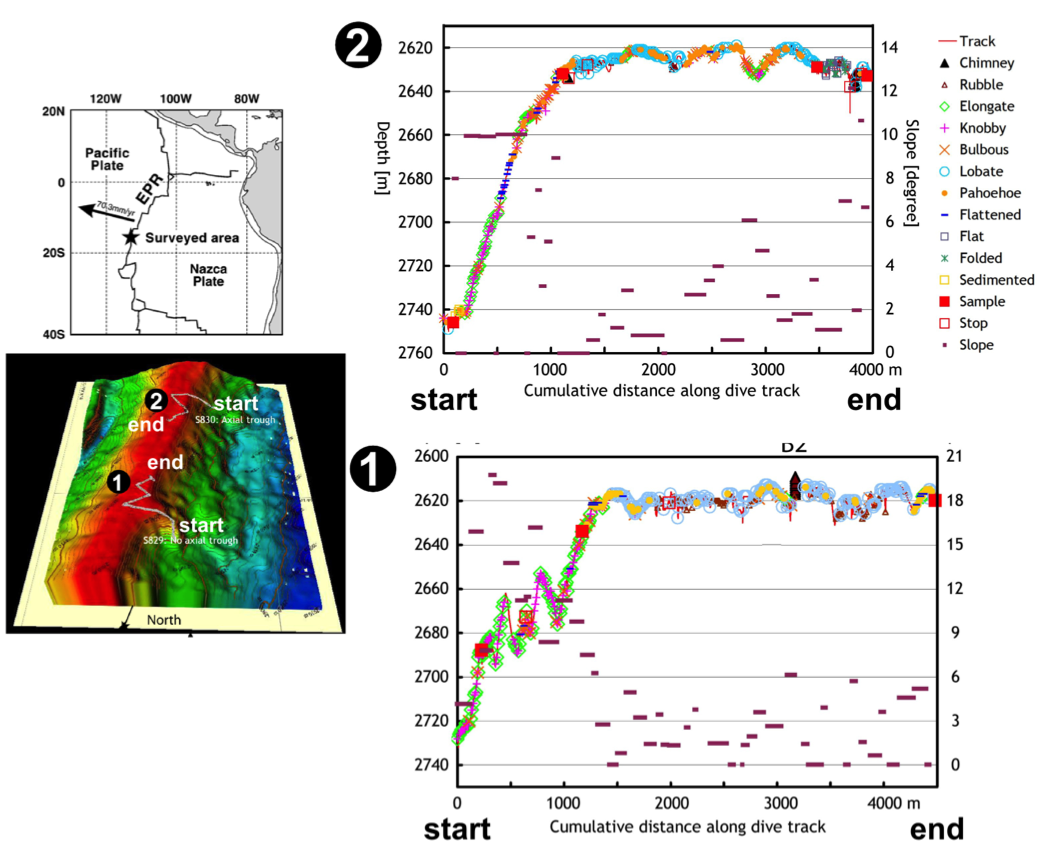
\includegraphics[width=0.9\textwidth]{TominagaUmino_G3_2010.png}
       {\scriptsize \citep{Tominaga2010}}
      \end{flushright}
    \end{minipage}
}


%%%%%%%%%%%%%%%%%%%%%%%%%%%%%%%%%%%%%%%%%%%%%%%%%%%%%%%%%%%%%%%%%%%%%%%%%%%%%%
  \headerbox{Hypotheses}{name=hypotheses,column=1,row=0,span=1}{
%%%%%%%%%%%%%%%%%%%%%%%%%%%%%%%%%%%%%%%%%%%%%%%%%%%%%%%%%%%%%%%%%%%%%%%%%%%%%%
{\large $\diamond$ Tensional strength of solidified lava}\\
    \begin{minipage}[t]{1.0\linewidth}
    \begin{multicols}{2}
``As a broad lobe encounters a steep slope, the gravitational forces increase the tension on the solid crust, causing the lobe to break apart into smaller `fingers' of lava. Conservation of mass dictates that the effusion rate of a small part of a lobe be less than the effusion rate of the entire lobe, so pillows are more likely to be generated as the lava flow breaks into smaller units.'' \citep{Gregg2003}.
    \end{multicols}
    \end{minipage}

{\large \vspace{0.3em} $\diamond$ Instability of viscous sheet flow down a slope}\\
    \begin{minipage}[t]{1.0\linewidth}
      \begin{center}
       \vspace{-0.5em}
       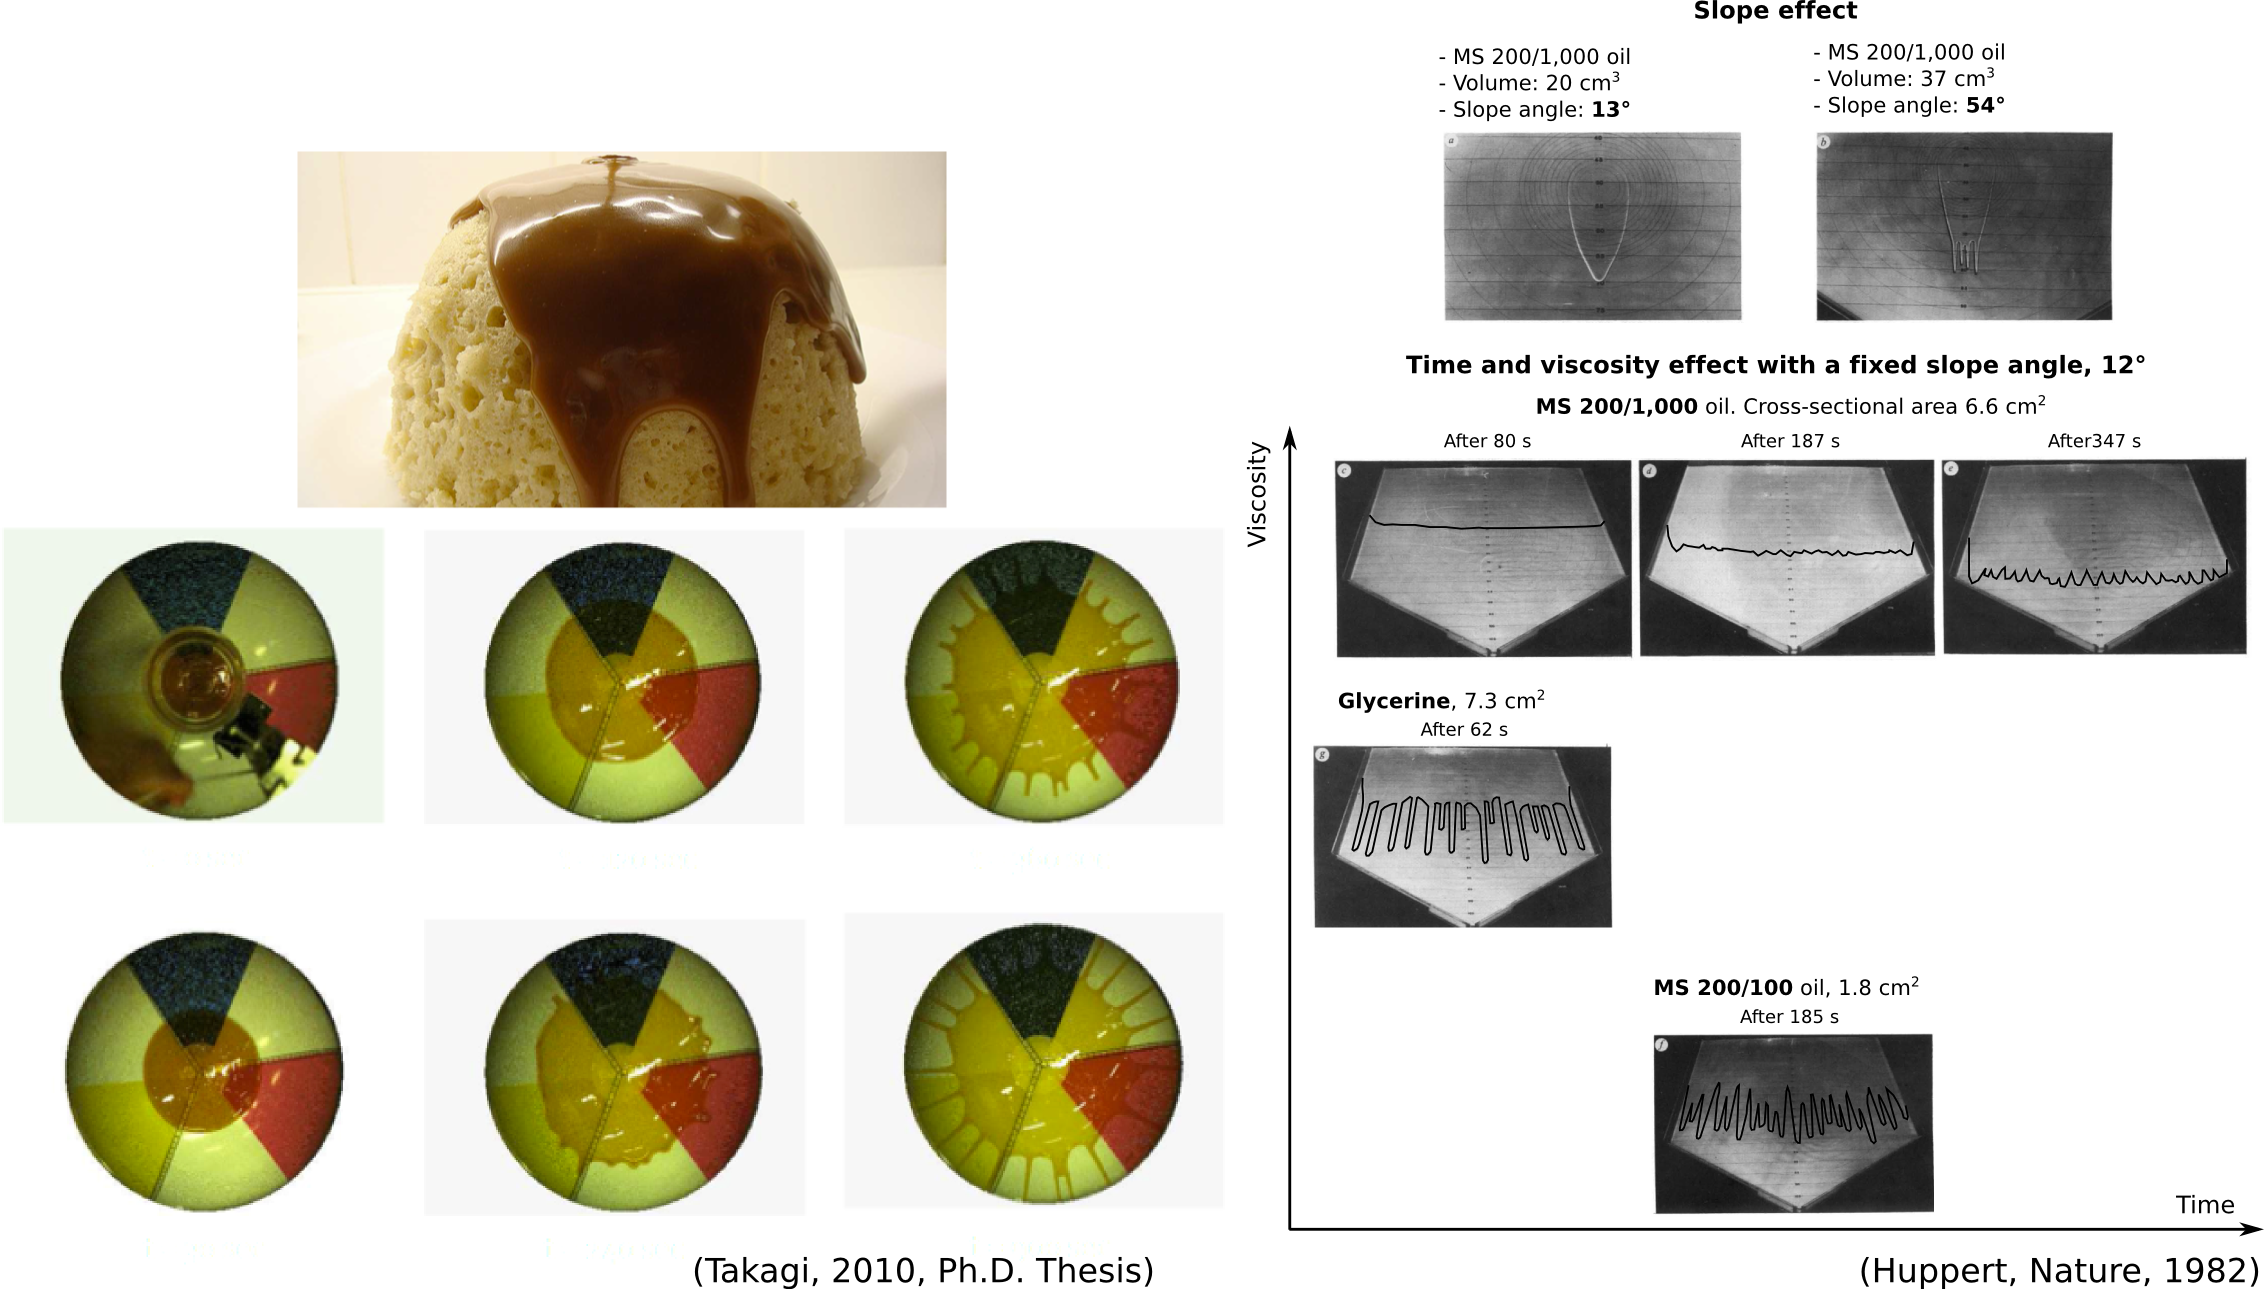
\includegraphics[width=0.85\textwidth]{instability.png}
      \end{center}
      \vspace{-1em}
      {\scriptsize (left) The radius of the sphere is 23 cm; kinematic viscosity and surface tension of the golden syrup is 4.5$\times$10$^{2}$ cm$^{2}$/s and 78 mN/m, respectively.}
    \end{minipage}
}

%%%%%%%%%%%%%%%%%%%%%%%%%%%%%%%%%%%%%%%%%%%%%%%%%%%%%%%%%%%%%%%%%%%%%%%%%%%%%%
  \headerbox{Numerical Approach}{name=approach,column=1,below=hypotheses,span=1}{
%%%%%%%%%%%%%%%%%%%%%%%%%%%%%%%%%%%%%%%%%%%%%%%%%%%%%%%%%%%%%%%%%%%%%%%%%%%%%%
We treat basaltic lava flow as \textbf{Stokes flow} with \textbf{temperature-sensitive viscosity} and \textbf{yielding}. \\\vspace{-1.0em}

{\large $\diamond$ Candidate Codes}\\
\begin{center}
\begin{minipage}[t]{1.0\linewidth}
\vspace{-3.0em}
\small
\begin{multicols}{2}
\begin{itemize}\setlength{\itemsep}{0mm}
\item \textbf{GALE}: 3D particle-in-cell FE code for multiphase Stokes flow  (\url{http://www.geodynamics.org/cig/software/gale}).
\item \textbf{pTatin3d}: A scalable, matrix-free, marker-and-cell-based 3D multiphase Stokes flow solver (May et al., to be submitted).
\item \textcolor{gray}{LavaSIM: A Simple Marker And Cell (SMAC) code for lava flow simulation \citep{Hidaka2005}.}
% May, D. A., Brown, J. and Le Pourhiet, L. 2013. A scalable, matrix-free Stokes discretisation for geodynamic applications, to be submitted to Computational Methods in Applied Mechanics and Engineering.
\end{itemize}
\end{multicols}
\end{minipage}
\end{center}

{\large $\diamond$ Model Setup}\\
\vspace{-2.0em}
\begin{center}
   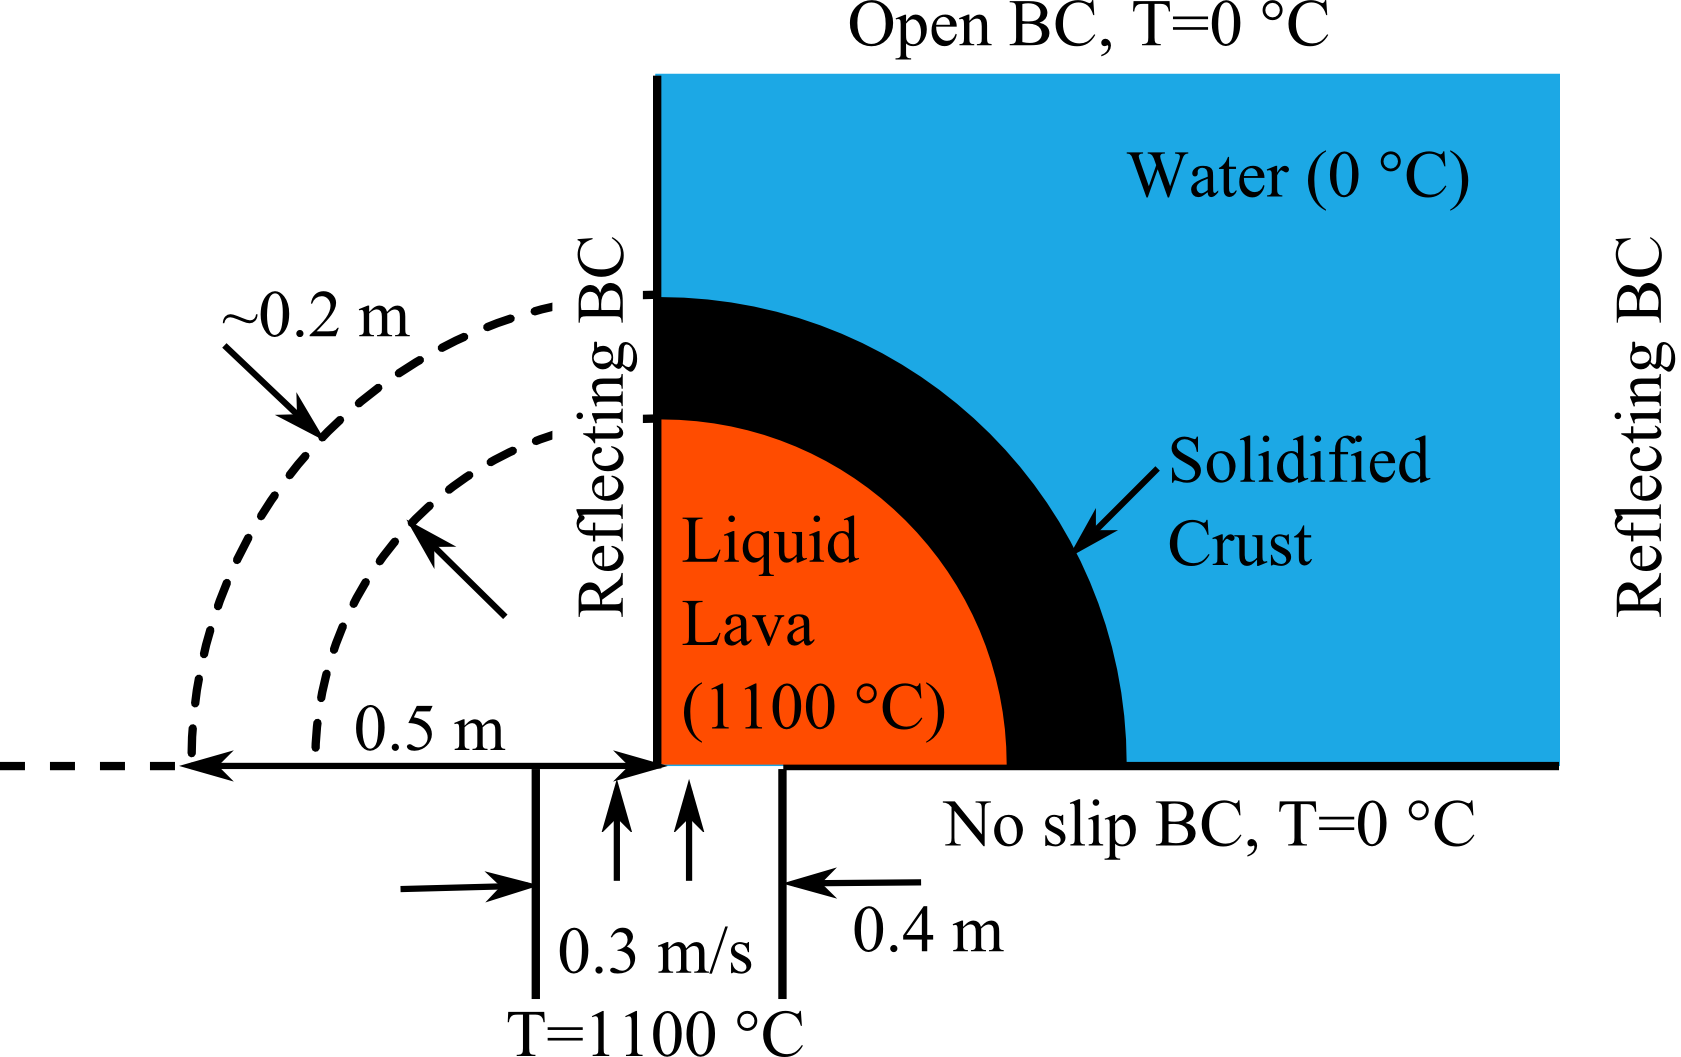
\includegraphics[width=0.5\textwidth]{Gale_model_setting.png} 
\end{center}
\begin{minipage}[t]{1.0\linewidth}
   \noindent
   \vspace{-3.0em}
   \scriptsize
   \begin{multicols}{2}
   \begin{itemize}[leftmargin=1.5em]\setlength{\itemsep}{0em}
      \item Density of basaltic lava: 2800 kg/m$^{3}$. 
      \item Rheology from \citep{Griffiths2000}
      \vspace{-1em}
      \begin{itemize}[leftmargin=0.5em] %\setlength{\itemindent}{-2em}
         \item Viscosity:
         \setlength{\abovedisplayskip}{0.2em}
         \setlength{\belowdisplayskip}{0.2em}
         \begin{equation*}
            \eta(T,\phi) = \eta_{0} (1.0-\phi/\phi_{max})^{-2.5}\exp[ -\gamma(T_{e}-T) ],
            \label{eq:basalt viscosity}
         \end{equation*}
         where $\eta_{0}$ is the reference viscosity (50 Pa$\cdot$s) at the vent temperatre, $T_{e}$ (=1100 $^{\circ}$C), $\phi_{max}$ is the maximum crystal fraction ($\sim$0.68) that allows flow and $\gamma$ is a constant (0.04). 

       \item The volume fraction of crystal, $\phi$:
       \begin{equation*}
          \phi(T) = \phi_{0} + \phi_{f}(T_{e}-T)/(T_{e}-T_{s}),
       \end{equation*}
       where $\phi_{0}$ is the initial crystal fraction at vent, which is zero, $\phi_{f}$ is the further increment during flow satisfying $\phi_{0}+\phi_{f} = \phi_{max}$ and $T_{s}$ is the solidus (600 $^{\circ}$C). According to the above two expressions, viscosity grows from $\sim$10 Pa$\cdot$s to 10$^{5}$ Pa$\cdot$s as temperature decreases to the ambient value (0 $^{\circ}$C). 

       \item Drucker-Prager plasticity: With internal friction angle set to be zero, only cohesion-like yield stress ($S_{y}$) is set to be temperature-dependent, reflecting the cooling effect \citep{Miyamoto1998}:
          \begin{equation*}
             S_{y}(T) = 10^{11.59-0.0089T},
          \end{equation*}
          where $T$ is in $^{\circ}$C.
     \end{itemize}
   \end{itemize}
   \end{multicols}
\end{minipage}
}

%%%%%%%%%%%%%%%%%%%%%%%%%%%%%%%%%%%%%%%%%%%%%%%%%%%%%%%%%%%%%%%%%%%%%%%%%%%%%
  \headerbox{2D Results}{name=2dresults,column=2,row=0,span=1}{
%%%%%%%%%%%%%%%%%%%%%%%%%%%%%%%%%%%%%%%%%%%%%%%%%%%%%%%%%%%%%%%%%%%%%%%%%%%%%%
\begin{minipage}[t]{1.0\textwidth}
%  \vspace{-2em}
{\large $\diamond$ Effects of slopes}
  \begin{flushright}
   \includegraphics[width=0.95\textwidth]{Gale_pTatin3d_flat_results.png} 
   %\includegraphics[width=0.95\textwidth]{Gale_pTatin3d_slope_results.png}
  \end{flushright}
\end{minipage}
\noindent
\begin{minipage}[c]{1.0\textwidth}
\begin{minipage}[t]{0.49\linewidth}
{\large $\diamond$ Effects of effusion rates}\\    
   \begin{center}
     \vspace{-1.5em}
     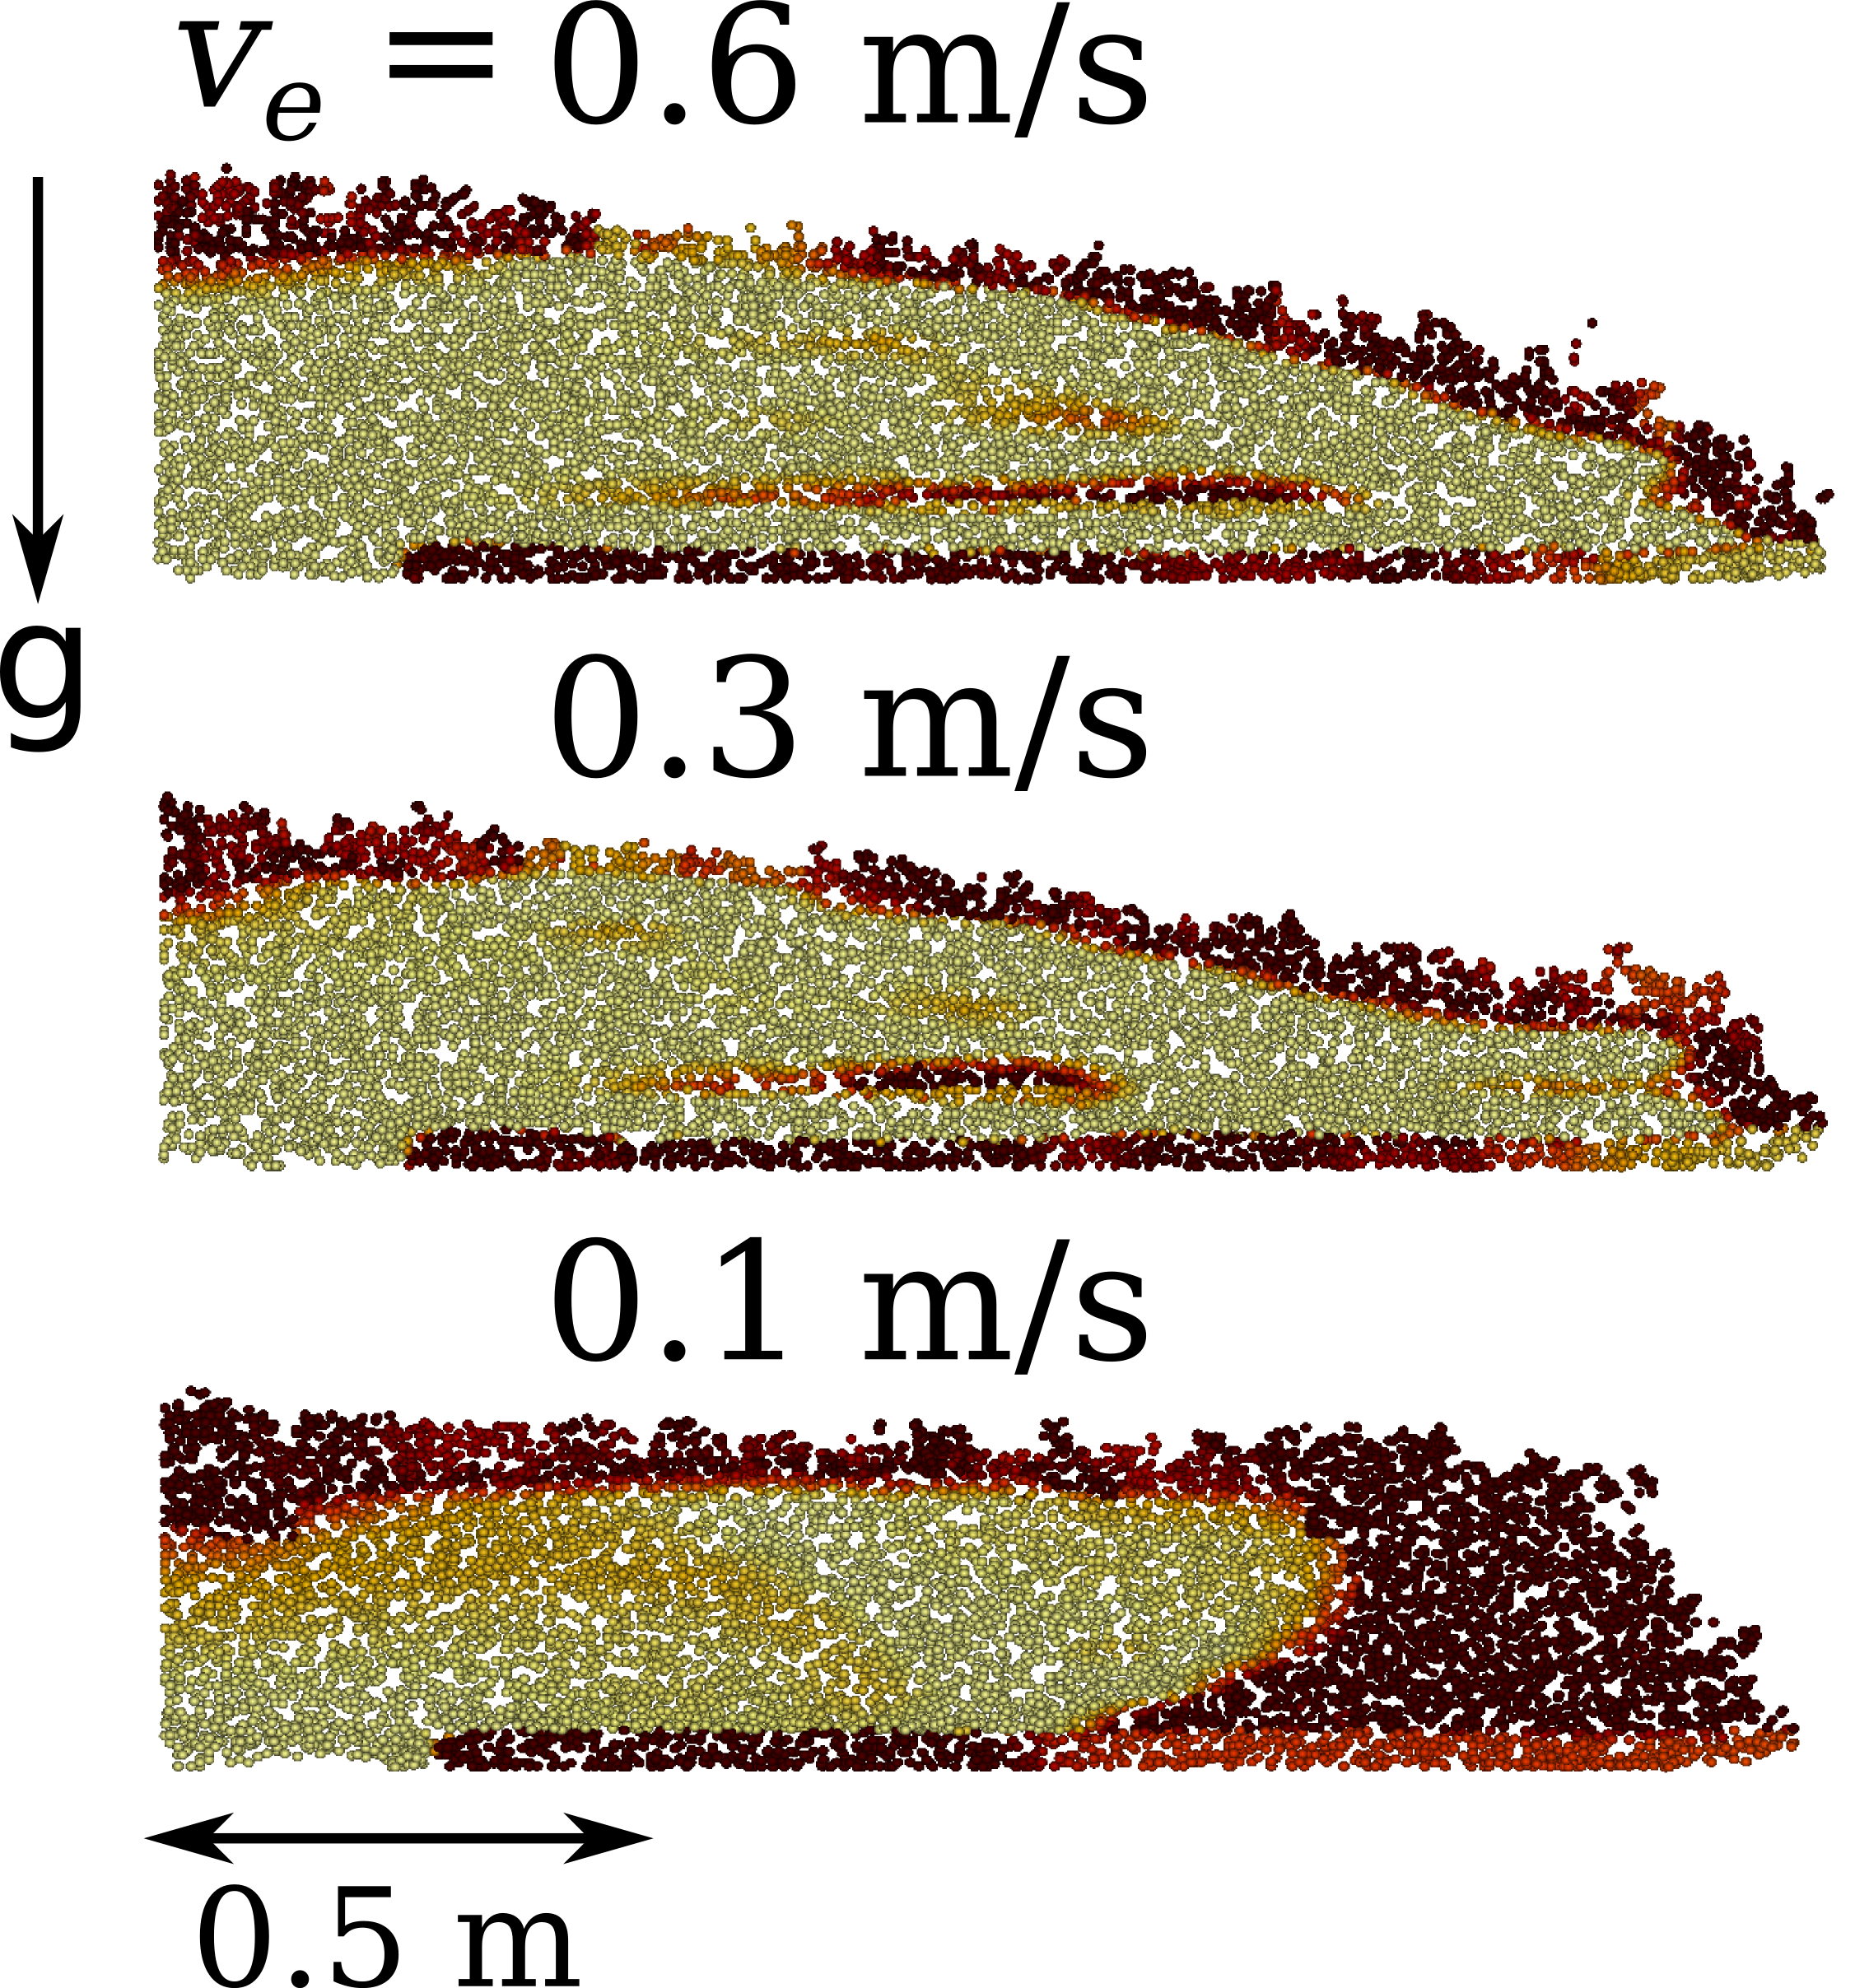
\includegraphics[width=0.7\textwidth]{Gale_effusion_rate.png}
     \vspace{0.5em}
   \end{center}
\end{minipage}%
\begin{minipage}[t]{0.49\linewidth}
\small
\begin{itemize}
  \item The two codes were run with some differences in the minimum viscosity and heat diffusivity of the ``water'' phase.
  \item Probably due to those differences, qualitative behaviors of the two are differently, especially on the 45$^\circ$ slope.
  \item More careful benchmarking needs to be designed.
  \item Besides the validation of results, it turned out to be difficult to identify lava flow morphology in 2D models. 
  \item It seem particularly challenging to create and identify pillows in 2D models.
\end{itemize}
\end{minipage}
\end{minipage}

}
  
%%%%%%%%%%%%%%%%%%%%%%%%%%%%%%%%%%%%%%%%%%%%%%%%%%%%%%%%%%%%%%%%%%%%%%%%%%%%%%
  \headerbox{Preliminary 3D Models by pTatin3d}{name=summary,column=2,below=2dresults,span=1}{
%%%%%%%%%%%%%%%%%%%%%%%%%%%%%%%%%%%%%%%%%%%%%%%%%%%%%%%%%%%%%%%%%%%%%%%%%%%%%%
\begin{minipage}[t]{1.0\textwidth}
  \begin{center}
    \includegraphics[width=0.95\textwidth]{pTatin3d_3D_results.png}
  \end{center}
\end{minipage}

{\small
\begin{multicols}{2}
\begin{itemize} \setlength{\itemsep}{-0.2em}
  \item 64$\times$32$\times$64 Q2-P1 elements. 
  \item At each time step, requires approximately three newton iterations to converge until the residual $< 10^{-4}$.
  \item Each time step requires between $\sim320$ sec on 64 cores. Compute nodes are 410 nodes consist of four quad-core AMD Opteron 8380 CPUs and 32 GB.
  \item Memory requirement per core is $< 1024$ GB
  \item Viscosity contrast in models is 1e7
  \item Multi-grid solver provides $O(N)$ scaling: Lower resolution models with 32x16x32 Q2-P1 elements on 64 cores took $\sim40$ sec.
\end{itemize}
\end{multicols}
}


}


%%%%%%%%%%%%%%%%%%%%%%%%%%%%%%%%%%%%%%%%%%%%%%%%%%%%%%%%%%%%%%%%%%%%%%%%%%%%%
%   \headerbox{References}{name=references,column=2,span=1,below=summary}{
%     \bibliographystyle{Refs/agu08}
%     \bibliography{Refs/references}{}
%   }

  \headerbox{References}{name=references,column=2,span=1,below=summary}{
    \begin{center}
    \begin{minipage}[t]{0.93\linewidth}
      \vspace{-0.5em}
      \begin{multicols}{2}
        \tiny \vspace{-1.0em} \bibliographystyle{agu08}
        \renewcommand{\section}[2]{\vskip 0.0em}

\begin{thebibliography}{7} \setlength{\itemsep}{0em}
\providecommand{\natexlab}[1]{#1}
\expandafter\ifx\csname urlstyle\endcsname\relax
  \providecommand{\doi}[1]{doi:\discretionary{}{}{}#1}\else
  \providecommand{\doi}{doi:\discretionary{}{}{}\begingroup
  \urlstyle{rm}\Url}\fi

\bibitem[{\textit{Fink and Griffiths}(1990)}]{Fink1990}
Fink, J.~H., and R.~W. Griffiths (1990), {Radial spreading of viscous-gravity
  currents with solidifying crust}, \textit{Journal of Fluid Mechanics},
  \textit{221}, 485--509, \doi{10.1017/S0022112090003640}.

\bibitem[{\textit{Gregg and Fink}(1995)}]{Gregg1995}
Gregg, T. K.~P., and J.~H. Fink (1995), {Quantification of submarine lava-flow
  morphology through analog experiments}, \textit{Geology}, \textit{23}(1), 73,
  \doi{10.1130/0091-7613(1995)023<0073:QOSLFM>2.3.CO;2}.

\bibitem[{\textit{Gregg and Smith}(2003)}]{Gregg2003}
Gregg, T. K.~P., and D.~K. Smith (2003), {Volcanic investigations of the Puna
  Ridge, Hawai$^{\prime}$i: relations of lava flow morphologies and underlying
  slopes}, \textit{Journal of Volcanology and Geothermal Research},
  \textit{126}(1-2), 63--77, \doi{10.1016/S0377-0273(03)00116-1}.

\bibitem[{\textit{Griffiths}(2000)}]{Griffiths2000}
Griffiths, R. (2000), {The dynamics of lava flows}, \textit{Annual review of
  fluid mechanics}, \textit{32}(1), 477--518.

\bibitem[{\textit{Hidaka et~al.}(2005)\textit{Hidaka, Goto, Umino, and
  Fujita}}]{Hidaka2005}
Hidaka, M., A.~Goto, S.~Umino, and E.~Fujita (2005), {VTFS project: Development
  of the lava flow simulation code LavaSIM with a model for three-dimensional
  convection, spreading, and solidification}, \textit{Geochemistry Geophysics
  Geosystems}, \textit{6}(7), Q07,008, \doi{10.1029/2004GC000869}.

\bibitem[{\textit{Miyamoto and Sasaki}(1998)}]{Miyamoto1998}
Miyamoto, H., and S.~Sasaki (1998), {Numerical simulations of flood basalt lava
  flows: Roles of parameters on lava flow morphologies}, \textit{Journal of
  geophysical research}, \textit{103}(B11), 27,489--27,502.

\bibitem[{\textit{Tominaga and Umino}(2010)}]{Tominaga2010}
Tominaga, M., and S.~Umino (2010), {Lava deposition history in ODP Hole 1256D:
  Insights from log-based volcanostratigraphy}, \textit{Geochemistry Geophysics
  Geosystems}, \textit{11}(5), 1--19, \doi{10.1029/2009GC002933}.

\end{thebibliography}

   

    \end{multicols}
  \end{minipage}
  \end{center}

  }

\end{poster}%
%
\end{document}
